% !TEX root = /home/computer/ucsc/master-2/quarter-2/advanced-fluids/master.tex
\assignment{3}{Thu 27 Jan 2022 10:59}{Assignment 3}
\subsectionfont{\fontsize{10}{10}\selectfont}

\graphicspath{{./assignment_03/figures/}}

\section{Wave packet approximation}%
\label{sec:wave_packet_approximation}

Taking the dot product of the momentum equation with the velocity vector ${\bf
u}$, and making the appropriate assumptions on the background state, we get an
energy equation in the form 

\begin{equation} \label{eq:1}
  \diffp[]{E_{T}}{t} + \nabla \cdot ( \text{Flux})
  = \frac{\tilde{p}^2}{2 \bar \rho } \diffp[]{}{t} \left( \frac{1}{c^2}\right)
\end{equation}

where total energy $E_{T}$ is the sum of kinetic energy, $ E_{K}=\bar \rho \frac{
\tilde{ {\bf u}}^2}{2}$, and compressional energy, $ E_{P}=\frac{\tilde{p}^2}{2 \bar
\rho c^2}$. Using a similar wavepacket approximation for velocity, we relate $U
( {\bf X}, T)$ to the amplitude $ A ( {\bf X}, T)$ using the momentum equation,
and we find there is an equipartition between kinetic and accoustic energies in
the wave packet amplitude solution

\[
  E_{T} = E_{K} + E_{P} =  \frac{| A|^2}{2 \bar \rho c^2} + \frac{| A|^2}{2 \bar \rho c^2}
.\] 

So, we seek a similar equation to (\ref{eq:1}). Multiplying the evolution
equation for amplitude with $A^{*}/ \bar \rho c^2$, we get

\begin{equation} \label{eq:2}
  \frac{1}{\bar \rho c^2} \diffp[]{|A|^2}{T} + \frac{1}{\bar \rho c^2} {\bf
  c_{g}} \cdot \nabla _{\epsilon }|A|^2 = -\frac{|A|^2}{\bar \rho kc} \left[
  \diffp[]{}{T} \left(\frac{\omega}{c^2}\right) + \nabla _{\epsilon } \cdot {\bf
  k} \right]
\end{equation}

where $k = | {\bf k}|$ is the norm of the wavevector, and ${\bf c_{g}}=
\frac{c^2}{\omega }{\bf k}$, is the group velocity vector. We want

\begin{equation} \label{eq:3}
  \diffp[]{}{T} \left( \frac{|A|^2}{\bar \rho c^2}\right) + \nabla _{\epsilon
  } \cdot \left( {\bf c_{g}} \frac{|A|^2}{\bar \rho c^2}\right)
\end{equation}

using the chain rule we recover (\ref{eq:2}) with additional terms so we add
this in and we get

\begin{align*}
  \diffp[]{}{T} \left( \frac{|A|^2}{\bar \rho c^2}\right) + \nabla _{\epsilon
  } \cdot \left( {\bf c_{g}} \frac{|A|^2}{\bar \rho c^2}\right) = -\frac{|A|^2}{\bar \rho kc} \left[
  \diffp[]{}{T} \left(\frac{\omega}{c^2}\right) + \nabla _{\epsilon } \cdot {\bf
  k} \right] \\
  + |A|^2 \diffp[]{}{T} \left(\frac{1}{\bar \rho c^2}\right) + |A|^2
  \nabla _{\epsilon } \cdot \left(\frac{{\bf c_{g}}}{\bar \rho c^2}\right)
\end{align*}

using the chain rule on the RHS for $ \diffp[]{}{T}$ terms and pulling out
$ \frac{|A|^2}{\bar \rho }$, and rearranging and using the dispersion relation
$w = ck$

\begin{gather*}
    \frac{|A|^2}{\bar \rho } \left[ \frac{1}{c^2} \cancelto{0}{\diffp[]{}{T} \left( \frac{1}{\bar \rho } \right)} + \cancel{\diffp[]{}{T} \left( \frac{1}{c^2} \right)} + \frac{1}{\bar c^2} \nabla _{\epsilon } \cdot {\bf
    c_{g}} + \frac{\bar \rho}{\bar \rho} {\bf c_{g}} \cdot \nabla _{\epsilon }\frac{1}{c^2} \right] \\
\frac{|A|^2}{\bar \rho } \left[ - \frac{1}{\omega c^2}\diffp[]{\omega }{T}
  - \cancel{\frac{\omega}{\omega}\diffp[]{}{T} \left( \frac{1}{c^2}\right)} - \frac{1}{\omega
}\nabla_{\epsilon } \cdot {\bf k}  \right]
\end{gather*}

$\diffp[]{}{T} \frac{1}{\bar \rho }$ goes to zero and $\nabla _{\epsilon
} \frac{1}{\bar \rho c^2} = \frac{1}{\bar \rho }\nabla _{\epsilon
} \frac{1}{c^2}$ if we make the assumption that $\bar \rho $ is constant. Using
\[
\frac{1}{c^2}\nabla _{\epsilon }\cdot {\bf c_{g}} + {\bf c_{g}} \cdot \nabla
_{\epsilon }\frac{1}{c^2} = \nabla _{\epsilon } \cdot \left( \frac{{\bf
c_{g}}}{c^2} \right)
.\] 

we have
\[
  \frac{|A|^2}{\bar \rho } \left[\nabla _{\epsilon } \cdot \left( \frac{{\bf
  c_{g}}}{c^2} \right) - \frac{1}{\omega c^2} \diffp[]{\omega }{T}
- \frac{1}{\omega }\nabla _{\epsilon }\cdot {\bf k} \right]
.\] 

using ${\bf c_{g}} = \frac{c^2}{\omega } {\bf k}$, then

\begin{align*}
  \nabla _{\epsilon } \cdot \left( \frac{{\bf
      c_{g}}}{c^2} \right) &= \nabla _{\epsilon } \cdot \left( \frac{{\bf k}}{\omega
  } \right) \\
  &= \frac{1}{\omega } \nabla _{\epsilon }\cdot {\bf k} + {\bf k} \cdot \nabla
  _{\epsilon } \frac{1}{\omega }
\end{align*}

putting this together

\begin{gather*}
  \frac{|A|^2}{\bar \rho } \left[\cancel{\frac{1}{\omega } \nabla _{\epsilon }\cdot {\bf k}} + {\bf k} \cdot \nabla
  _{\epsilon } \frac{1}{\omega } - \frac{1}{\omega c^2} \diffp[]{\omega }{T}
- \cancel{\frac{1}{\omega }\nabla _{\epsilon }\cdot {\bf k}} \right] \\
   = \frac{|A|^2}{\bar \rho } \left[{\bf k} \cdot \nabla
  _{\epsilon } \frac{1}{\omega } - \frac{1}{\omega c^2} \diffp[]{\omega }{T}
\right] \\
   = \frac{|A|^2}{\bar \rho \omega c^2 } \left[ \omega c^2{\bf k} \cdot \nabla
  _{\epsilon } \frac{1}{\omega } -  \diffp[]{\omega }{T}
\right] \\
\end{gather*}

Subbing ${\bf k} = \frac{\omega}{c^2}{\bf c_{g}}$, then

\[
\omega c^2{\bf k} \cdot \nabla
  _{\epsilon } \frac{1}{\omega } = \omega ^2 {\bf c_{g}} \cdot \nabla
  _{\epsilon } \frac{1}{\omega }
.\] 

using $\nabla _{\epsilon } \omega ^{-1} = -\frac{1}{\omega^2 } \nabla
_{\epsilon } \omega $, we get

\[
  -\frac{|A|^2}{\bar \rho \omega c^2 } \left[ {\bf c_{g}} \cdot \nabla
  _{\epsilon } \omega  +  \diffp[]{\omega }{T} \right]
.\] 

then using the dispersion relation $\omega = ck$, and the evolution equation
for $\omega $

\begin{align*}
  \diffp[]{\omega }{T} + {\bf c_{g}} \cdot \nabla
  _{\epsilon } \omega &= \left( \diffp[]{\Omega}{T} \right)_{{\bf k}} \\
                      &= k \diffp[]{c}{T} \qquad \text{for constant {\bf k}}
\end{align*}

we get

\begin{align*}
  &-\frac{|A|^2}{\bar \rho \omega c^2 } \left[k \diffp[]{c}{T} \right] \\
  &= -\frac{|A|^2}{\bar \rho c^3 } \left[ \diffp[]{c}{T} \right] \qquad  \omega = ck
\end{align*}

using $\diffp[]{c^{-2}}{T} = -\frac{2}{c^{3}} \diffp[]{c}{T}$, and putting
everything together, we finally get

\begin{equation}
  \boxed{\diffp[]{}{T} \left( \frac{|A|^2}{\bar \rho c^2}\right) + \nabla _{\epsilon
  } \cdot \left( {\bf c_{g}} \frac{|A|^2}{\bar \rho c^2}\right)
  = \frac{|A|^2}{2 \bar \rho } \diffp[]{}{T} \left( \frac{1}{c^2} \right)}
\end{equation}

\section{Application: A sound mirror}%
\label{sec:application_a_sound_mirror}


Considering the wave packet evolution equations for constant sound speed


\begin{gather}
  \diffp[]{{\bf k}}{T} + {\bf c_{g}} \cdot \nabla _{\epsilon } {\bf k} = 0 \label{eq:5}\\
  \diffp[]{\omega }{T} +  {\bf c_{g}} \cdot \nabla _{\epsilon } \omega  = 0 \label{eq:6}\\
  \diffp[]{A}{T} +  {\bf c_{g}}\cdot\nabla _{\epsilon } A  = - \frac{Ac}{2} \nabla
  _{\epsilon } \cdot \left( \frac{{\bf k}}{k} \right) \label{eq:7}
\end{gather}

then inside the first half sphere the divergence of the wavevector is positive

\begin{figure}[H]
    \centering
    \incfig{region1}
    \caption{region1}
    \label{fig:region1}
\end{figure}

in this region, before the sound hits the wall, the amplitude decreases while
being advected. We can see this from the RHS of (\ref{eq:7}).  Then using the
property (approximating the half sphere as a parabola), that rays emitted from
the focus go to infinity on parallel lines, then

\begin{figure}[H]
    \centering
    \incfig{region2}
    \caption{region2}
    \label{fig:region2}
\end{figure}

as the sound travels across the room, the amplitude is conserved as it is
advected. Finally, when the sound reaches the other half sphere, these parallel
lines are then focused as the amplitude grows and converges at a point where
the other person stands.


\begin{figure}[H]
    \centering
    \incfig{region3}
    \caption{region3}
    \label{fig:region3}
\end{figure}

If the speaker were to turn around and speak towards the person across the
room, the amplitude would likely dissipate before reaching it's destination.

\section{Diffraction of sound waves}%
\label{sec:diffraction_of_sound_waves}

Initially we have (\ref{eq:5}), (\ref{eq:6}), and (\ref{eq:7}) for the
evolution of the wave packet with constant sound speed, where $\omega
=\omega_0$ is advected without change, and dispersion relation $\omega_0^2
= c_0^2|{\bf k}|^2$. The evolution equations for non-constant sound speed

\begin{gather}
  \diffp[]{\omega }{T} + {\bf c_{g}}\cdot \nabla _{\epsilon } = \left(
  \diffp[]{\Omega}{T}\right)_{{\bf k}} = k \diffp[]{c_{s}}{T} = 0 \\
  \diffp[]{{\bf k}}{T} + {\bf c_{g}}\cdot \nabla _{\epsilon } = - (\nabla
  _{\epsilon }\Omega)_{{\bf k}} = -k \nabla _{\epsilon }c_{s}(X,Y) \\
  \diffp[]{A}{T} + {\bf c_{g}}\cdot \nabla _{\epsilon }A
  = - \frac{Ac_{s}^2}{2\omega } \left[ \diffp[]{}{T} \left(
  \frac{\omega}{c_{s}^2}\right) + \nabla _{\epsilon }\cdot {\bf k} \right]
\end{gather}


Since $c_{s}$ doesn't depend on time, $\omega = \omega_0$ is still conserved.
Then from the dispersion relation $\omega ^2 = c_{s}^2(X,Y) |{\bf k}|^2$ for waves
coming from $Y \rightarrow + \infty $ in the region of the sound speed anomoly, we have

\[
{\bf k} = \begin{pmatrix}
  k_{x} \\ k_{y}
\end{pmatrix} = \begin{pmatrix}
  0 \\ k_{y}
\end{pmatrix}
.\] 

so
\begin{align*}
  \omega_0 ^2 &= c^2(X,Y) k_{y}^2 \\
  \implies k_{y}^2  &= \frac{\omega_0 ^2}{c_{s}^2(X,Y)}
\end{align*}

for $c_{s}(X,Y) = c_0 + (\Delta c)e^{ -\frac{X^2+Y^2}{2}}$

\begin{figure}[H]
  \centering
  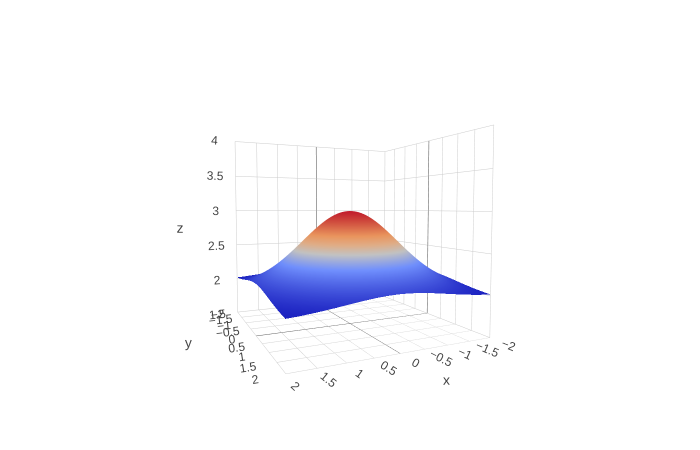
\includegraphics[width=0.8\linewidth]{sound_anomaly.png}
  \caption{Sound anomaly}%
  \label{fig:sound_anomaly}
\end{figure}

we have the following figure for how wave paths change

\graphicspath{{/home/ucsc/current-course/figures/}}
\begin{figure}[H]
    \centering
    \incfig{paths}
    \caption{paths}
    \label{fig:paths}
\end{figure}

Hence The $y$ component of ${\bf k}$ slows down as it approaches the area where
the sound speed increases, and we can see roughly how much it slows down by
drawing contour lines of the graph of $c_{s}$. On the other hand, if $\Delta
c <0$, the vectors ${\bf k}$ speed up

\begin{figure}[H]
    \centering
    \incfig{paths2}
    \caption{paths2}
    \label{fig:paths2}
\end{figure}

\section{Gravity waves wave packet equations}%
\label{sec:gravity_waves_wave_packet_equations}

Governing equation for internal gravity waves
\[
\diffp[2]{}{t} \left( \nabla ^2 \phi \right) = - \diffp[]{}{x} \left( N^2
\left( \diffp[]{\phi}{x}\right)\right)
.\] 

with ${\bf k} = \nabla \theta $ and $ \omega = - \diffp[]{\theta }{t}$. The
wave packet approximation

\[
  \phi = A(X,Z,T) e^{i \theta (x,z,t)}
.\] 

then
\[
\nabla \phi = \epsilon \nabla Ae^{i \theta } + i \nabla \theta Ae^{i \theta }
.\] 
\[
\nabla ^2\phi = \epsilon i \nabla A \nabla \theta e^{i \theta } + \epsilon
i \nabla ^2 \theta Ae^{i \theta } +  \epsilon i \nabla \theta \nabla A e^{i
\theta } - (\nabla \theta )^2 A e^{i \theta }
.\] 

$\dots$

\section{Gravity waves in a linearly stratified medium}%
\label{sec:gravity_waves_in_a_linearly_stratified_medium}

$N = aZ$, so evolution equation for $\omega $ is conserved, where dispersion
relation $\omega = \Omega = \pm \frac{k_{x}}{k}N(Z)$
\[
  \diffp[]{\omega }{T} + {\bf c_{g}}\cdot \nabla _{\epsilon
  } \omega = \diffp[]{\Omega}{T} = 0
.\] 

so set $\omega = \omega_0$, then ray paths can be found from
\[
  \diff[]{Z}{X} = \frac{{\bf c_{g}}\cdot {\bf e_{z}}}{{\bf c_{g}}\cdot {\bf
  e_{x}}} = \left( \frac{N(Z)^2}{\omega_0^2} - 1\right)^{-\frac{1}{2}}
.\] 

where group speed ${\bf c_{g}} = \frac{N}{k} \left( {\bf e_{x}} - k_{x}
\frac{{\bf k}}{k^2}\right)$, then we want to integrate

\[
  \left(\frac{a^2Z^2}{\omega_0} - 1\right)^{\frac{1}{2}} dZ = dX
.\] 

using the change of variable $\sec^2(\theta ) = \frac{a^2Z^2}{\omega_0}$, we
get
\[
  X(\theta ) = \frac{\sqrt{\omega_0}}{a}\int {\sec \theta \tan^2 \theta } \: d{\theta } 
.\] 

with solution
\[
  X(\theta ) = \frac{\sqrt{\omega_0}}{2a} \left( \tan \theta \sec \theta
  - \tanh^{-1} (\sin \theta ) \right)
.\] 

\graphicspath{{./assignment_03/figures/}}
\begin{figure}[H]
  \centering
  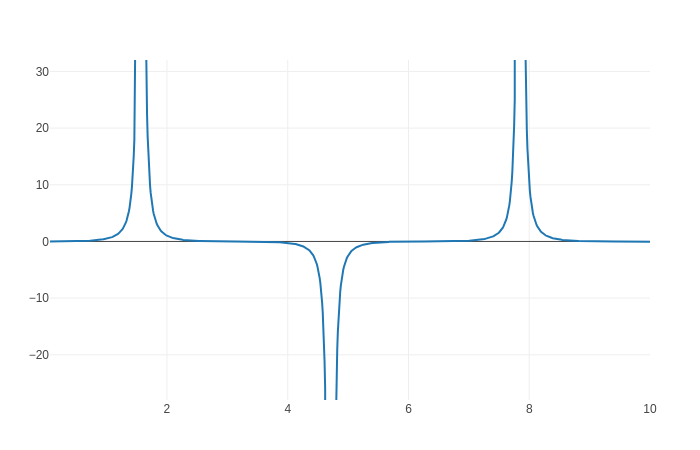
\includegraphics[width=0.8\linewidth]{plot.png}
  \caption{Plot}%
  \label{fig:plot}
\end{figure}
